\documentclass[tikz,border=10pt]{standalone}
\usepackage{tikz}
\usepackage{amsmath}
\usetikzlibrary{decorations.pathmorphing}

\begin{document}
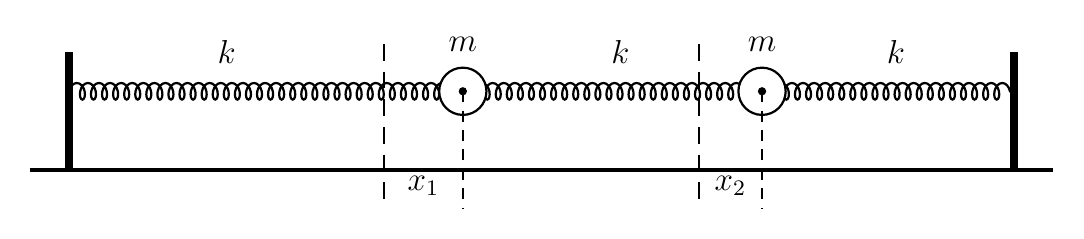
\begin{tikzpicture}[
    % 弹簧样式（波浪线）
    spring/.style={
        thick,
        decorate,
        decoration={coil, aspect=0.6, segment length=4pt, amplitude=3pt}
    },
    % 两端墙壁样式
    wall/.style={line width=3pt},
    % 底部基准线样式
    baseline/.style={thick, line width=1.5pt},
    % 质点和圆圈样式
    mass/.style={thick, draw, circle, minimum size=0.6cm, inner sep=0pt, fill=white},
    % 长虚线样式（用于平衡位置，稍疏）
    eqline/.style={thick, dashed, dash pattern=on 6pt off 4pt},
    % 短虚线样式（用于当前位置，稍密）
    posline/.style={thick, dashed, dash pattern=on 4pt off 3pt},
    % 字体大小
    label/.style={font=\large}
]

    % 1. 绘制底部基准线
    \draw[baseline] (-0.5, 0) -- (12.5, 0);

    % 2. 绘制左右两端墙壁
    \draw[wall] (0, 0) -- (0, 1.5);
    \draw[wall] (12, 0) -- (12, 1.5);

    % 3. 定义各个关键坐标
    \def\height{1.0}      % 质心高度（弹簧所在高度）
    \def\topYEq{1.6}      % 平衡位置虚线的顶端（高于弹簧）
    \def\topYPos{1.0}     % 当前位置虚线的顶端（从质心开始）
    \def\botY{-0.5}       % 四条竖线的共同底端（严格对齐且缩短）
    \def\labelY{-0.2}     % 广义坐标标签的垂直位置（调高）
    
    % 质点1：平衡位置在4.0，当前位置在5.0
    \def\eqXOne{4.0}
    \def\posXOne{5.0}
    
    % 质点2：平衡位置在8.0，当前位置在9.0
    \def\eqXTwo{8.0}
    \def\posXTwo{8.8}

    % 4. 绘制三个弹簧（连接到质点的当前位置）
    \draw[spring] (0, \height) -- (\posXOne, \height);          % 左侧弹簧
    \draw[spring] (\posXOne, \height) -- (\posXTwo, \height);    % 中间弹簧
    \draw[spring] (\posXTwo, \height) -- (12, \height);          % 右侧弹簧

    % 5. 绘制两个质点
    \node[mass] (m1) at (\posXOne, \height) {};
    \fill (\posXOne, \height) circle (1.5pt); 
    
    \node[mass] (m2) at (\posXTwo, \height) {};
    \fill (\posXTwo, \height) circle (1.5pt);

    % 6. 绘制广义坐标的竖线（全部为虚线，下端对齐）
    % --- 质点1 ---
    \draw[eqline]  (\eqXOne, \topYEq)  -- (\eqXOne, \botY);   % 平衡位置：长虚线
    \draw[posline] (\posXOne, \topYPos) -- (\posXOne, \botY);  % 当前位置：短虚线（从质心开始）
    \node[label] at ({(\eqXOne + \posXOne)/2}, \labelY) {\(x_1\)}; 

    % --- 质点2 ---
    \draw[eqline]  (\eqXTwo, \topYEq)  -- (\eqXTwo, \botY);   % 平衡位置：长虚线
    \draw[posline] (\posXTwo, \topYPos) -- (\posXTwo, \botY);  % 当前位置：短虚线（从质心开始）
    \node[label] at ({(\eqXTwo + \posXTwo)/2}, \labelY) {\(x_2\)}; 

    % 7. 添加顶部文字标注
    % 弹簧劲度系数 k
    \node[label] at (2.0, 1.5) {\(k\)}; 
    \node[label] at (7.0, 1.5) {\(k\)}; 
    \node[label] at (10.5, 1.5) {\(k\)}; 

    % 质点质量 m
    \node[label] at (\posXOne, 1.6) {\(m\)};
    \node[label] at (\posXTwo, 1.6) {\(m\)};

\end{tikzpicture}
\end{document}